% Dokument:
\documentclass[a4paper,10pt,twocolumn]{article}
\usepackage[utf8]{inputenc}
%\usepackage[norsk]{babel}
\usepackage{hyperref}

% Formatering:
\usepackage{geometry,amsthm,blindtext}
\setlength{\parindent}{3mm}
\setlength{\parskip}{1.8mm}
% Symboler
\usepackage[geometry]{ifsym}
% Matematikk:
\usepackage{amsmath,mathtools,amsfonts,xparse,physics,esint,mathrsfs,nicefrac,siunitx}
% Kode:
\usepackage{verbatim,listings,algpseudocode}
% Tekst:
\usepackage{textcomp,varioref,enumerate,bbold}
% Figurer:
\usepackage{graphicx,subcaption,float,dcolumn,multirow}
\usepackage[section]{placeins}
% Farge:
\usepackage{xcolor}

% Dcolumn-kolonner
\newcolumntype{,}{D{,}{{,}}{2}}
\newcolumntype{=}{D{=}{=}{-1}}
\newcolumntype{.}{D{.}{{.}}{2}}
\newcolumntype{C}{>{$}c<{$}}

% Listings-Instillinger
	\lstset{
	% Språk
	language=c++,
	% Farge
	backgroundcolor=	\color[rgb]{0.9,0.9,0.9},
	keywordstyle=		\color[rgb]{0,0,1},
        	commentstyle=		\color[rgb]{0.133,0.545,0.133},
        	stringstyle=		\color[rgb]{0.627,0.126,0.941},
	numberstyle=\tiny	\color[rgb]{0.5,0.5,0.5},
        	rulecolor=			\color{black},
	% Tekst:
	basicstyle=\scriptsize,
	showspaces=false,
	showstringspaces=false,
	showtabs=false,
	% Spesialtegn
	extendedchars=true,
        	literate=	{æ}{{\ae}}1 	{ø}{{\o}}1 		{å}{{\r a}}1 
		  	{≤}{{$\leq$}}1 	{≥}{{$\geq}}1	{–}{{$-$}}1		{~}{{\tiny{$\sim$}}}1,
        	% Format
	frame=single,
	aboveskip={1.5\baselineskip},
	breaklines=true,
	columns=fixed,
	numbers=left,
	numbersep=5pt,
	stepnumber=1,
	tabsize=4, 
	% ... 
        	upquote=true,
        	prebreak = \raisebox{0ex}[0ex][0ex]{\ensuremath{\hookleftarrow}},
        	identifierstyle=\ttfamily
        	}
	
% Nummerering:
%\renewcommand{\thesection}{\arabic{section}}		% Nummer i "section"
%\renewcommand{\thessubection}\arabic{subsection}}	% Nummer i "subsection"
%\renewcommand{\thesection}{\alph{section}}			% Bokstaver i ''section''
%\renewcommand{\thesubsection}{\alph{subsection}}	% Bokstaver i ''subsection''

% Egendefinerte kommandoer:
	% Snarveier
	\newcommand*{\eqset}[1]{\begin{dcases}#1\end{dcases}}
	\newcommand*{\Qfig}[3]{\begin{figure}[ht]	\centering \includegraphics[#2]{#1} \caption{#3} \end{figure} }
	% Tegn
	\newcommand{\point}{\varointclockwise}	% integral med klokken
	\newcommand{\noint}{\ointctrclockwise}	% integral mot klokken
	\newcommand{\ee}[1]{\!\times\!\!10^{#1}} 	% 10 i #1-te
	\newcommand{\un}[1]{\,\si{#1}}		% enheter
	\newcommand{\e}[1]{\mathrm{e}^{#1}}	% exp()
	\newcommand{\ci}{\dot{\iota\!\:}}		% kompleks i
	% misc
	\newcommand{\note}[1]{{\color{red}\quad[$\backslash!/$: #1]}}	% notater for dokument under arbeid
	\newlength{\txtsz}\makeatletter\setlength{\txtsz}{\f@size pt}\makeatother
	\newcommand{\insubsec}[1]{\par{\bf #1}}

% Åpning:
\title{Disease modeling with the SIRS model: comparison of a coupled differential equation and Monte Carlo based approach.}
\author{Johannes Sørby Heines}


% START
\begin{document}

\twocolumn[
\begin{@twocolumnfalse}
\maketitle
\begin{abstract}
We created an extendable code for performing Monte Carlo simulations of the SIRS model, and implemented modifications to model vital dynamics, seasonal variation in the transmission rate, and vaccination. The results were studied for different parameters in each case and compared to deterministic solutions of calculated with fourth order Runge-Kutta.   
The two approaches agree in most circumstances, but fluctuations in the Monte Carlo model may eradicate the disease completely when the number of infected gets close to zero. while this number can be arbitrarily small for the differential equations. 
Large disagreements between the two approaches are an effect of high dependence on the behaviour of individuals, and as such that a purely statistical model in no longer reliable.
\end{abstract}
\end{@twocolumnfalse}
]

\section{Introduction}

When determining how best  to respond to an outbreak of an infectious disease, being able to predict its spread throughout a given population is crucial.
Compartmental models classify the total population into different compartments – for example $S$: ``susceptible'', $I$: ``infected'' and $R$: ``recovered'' – and models the average transitions between these compartments. 

Such compartmental models have the advantage of being easily expandable both in terms of transitions and compartments, allowing for models tailored to a specific situation.   


In this project we study the SIRS model, in which the immunity gained by recovery is eventually lost, leading to a cyclic system. 

 
After introducing the SIRS model, we explain its implementation both as a system of coupled ordinary differential equations, and as a Monte Carlo system. 
We outline various improvements on the basic model and compare the two approaches in each case.   

%
%
%
\section{Theory}

All our code can be found at \url{https://github.com/johashei/ComputationalPhysics/tree/master/doc/Projects/2020/Project5/DiseaseModeling/project/code}.


\subsection{The SIRS model}
The basic SIRS model is a simple cyclic model of the evolution of a contagious disease in a population. It distinguishes three groups: susceptible (S), infected (I), and recovered (R), and models the transitions between these groups. 
These transitions are given by three quantities, namely the rates of transmission $\beta$, recovery $\gamma$, and immunity  loss $\lambda$. 

The parameter $\beta$ is defined as the average number of contacts per person per time, multiplied by the probability of infection in a contact between $S$ and $I$.
The parameters $\gamma$ and $\lambda$ are given by the inverse of the average recovery and immunity loss times, respectively.

The transitions are calculated assuming the three groups mix homogeneously. That is, the proportions of $S$, $I$ and $R$ in a subset of the population will be the same as in the population as a whole.  

%The average number of individuals being infected $(S\to I)$ in a time interval $\Delta t$ is  $\beta SI/N$. $The transmission rate $\beta$ is the product of the probability of transmission in a contact between $S$ and $I$ with the average number of contacts per person per time. $SI/N$ is the  
%The rate of infection is then given by $EPSI/N^2$, where $E$ is the average number of encounters per person per time, $SI/N^2$ is the fraction of contacts which are between a susceptible and an infected, and $P$ is the probability of infection in such an encounter. Usually, the two constants $E$ and $P$ are grouped together in a single parameter $\beta$. 
%The total number of new infected per time unit is then $\beta SI/N$.


The SIRS model can then be described by the following coupled differential equations \ref{eq:diff}, where each of the terms $\beta SI/N, \gamma I, \lambda R$ is the average number of individuals making the respective transitions $(S\to I), (I\to R), (R\to S)$ in one time unit.

\begin{subequations}\label{eq:diff}
\begin{align}
\dv{S}{t} &= \lambda R - \beta\frac{SI}{N},
\\ \dv{I}{t} &= \beta\frac{SI}{N} - \gamma I,
\\ \dv{R}{t} &= \gamma I - \lambda R.
\end{align} 
\end{subequations}


\subsection{Improvements to the SIRS model}

The SIRS model can easily be modified to include more effects, by changing or adding new terms to the differential equations \ref{eq:diff}. 
In this report, we will treat vital dynamics, seasonal variations and vaccination.

\textbf{Vital dynamics:}
The basic SIRS model described above assumes the population remains constant throughout the simulation. If the time scale of the epidemic is comparable to or longer than the average life span, the birth and death rates need to be accounted for. 
%Given adequate hospital facilities, many diseases won't be transmitted from a sick mother to the baby.  
If all newborns are susceptible to the disease, then the equilibrium will change even if the total population remains constant, as dying individuals in $I$ and $R$ are replaced with newborns in $S$. 
In addition, the disease may increase the death rate for the infected population. 

The corresponding differential equations are
\begin{subequations}
\begin{align}
\dv{S}{t} &= \lambda R - \beta\frac{SI}{N} - \mu S + \nu N,
\\ \dv{I}{t} &= \beta\frac{SI}{N} - \gamma I - \mu I - \mu_I I,\label{eq:cI}
\\ \dv{R}{t} &= \gamma I - \lambda R - \mu R,
\end{align}
\end{subequations}
where $\nu$ is the birth rate, $\mu$ is the death rate not related to the disease, and $\mu_I$ is the rate of death caused by the disease. 


\textbf{Seasonal variation:} For many common diseases, such as influenza or the common cold, the rate of transmission depends largely on the time of year. This can be caused by a multitude of factors which are not the subject of this report. 
On the simplest level, this variation can be modeled by adding a harmonic oscillation to the transmission parameter $\beta$:
\begin{equation}\label{eq:seasvar}
\beta(t) = A\cos(\omega t) + \beta_0,
\end{equation} 
where $A$ in the maximum deviation from $\beta_0$ and $\omega$ is the angular frequency of the seasonal variation.


\textbf{Vaccination:} Vaccination trains the immune system to respond to the infecting agent, creating a transition directly from $S$ to $R$.  As opposed to the previously discussed effects, the rate of vaccination typically depends little on the number of individuals in each compartment, and more on external factors like medical research and vaccination campaigns \cite{labtext}. 
We therefore model the vaccination rate as a simple function of time. 
\begin{subequations}
\begin{align}
\dv{S}{t} &= \lambda R - \beta\frac{SI}{N} - f(t),
\\ \dv{I}{t} &= \beta\frac{SI}{N} - \gamma I ,
\\ \dv{R}{t} &= \gamma I - \lambda R + f(t).
\end{align}
\end{subequations}

All these improvements, along with many others, can be combined to create a more realistic model for a given scenario.
 
\textbf{The basic reproduction number:}
All the improvements outlined above have analytical expressions for the equilibrium, which can be found by setting all three derivatives to zero. Particularly, $\dv*{I}{t} = 0$ gives the equilibrium $s^*$ for $S$. The number $R_0=N/s^*$ is then the basic reproduction number, and if it is larger than one, the disease will remain in the population. 
 
%
%
%
\section{Methods}

The goal of this project was threefold: to make an easily expandable code for the SIRS model,  to test the model's behaviour when including the effects described above, and to compare a Monte Carlo implementation to one based on coupled differential equations.

Since every state of the system depends on the previous state, neither algorithm is suited for vectorization nor parallelization. As we chose to focus on expandability rather than speed, this will not be discussed further in this report.  

\subsection{The coupled ODE approach}

The differential equations were solved using the Runge-Kutta 4 algorithm. This method is not symplectic, but has a global error $\order{h^4}$, where $h$ is the chosen step length. The algorithm is \cite{ODElecture}
%
\begin{algorithmic}
\For{$i=0:n-1$}
\State{$k_1 = h\cdot f(t_i,y_i)$}
\State{$k_2 = h\cdot f(t_{i+1/2}, y_i+\frac{k_1}{2})$}
\State{$k_3 = h\cdot f(t_{i+1/2}, y_i+\frac{k_2}{2})$}
\State{$k_4 = h\cdot f(t_{i+1}, y_i+k_3)$}
\State{$y_{i+1} = y_i + \frac{1}{6}(k_1+2k_2+2k_3+k_4)$}
\EndFor
\end{algorithmic}
%
When simulating a system of coupled differential equations, each line in calculated for every equation before moving to the next. 

The Runge-Kutta 4 method for the coupled differential equations was implemented with the python class \texttt{ODESolver} written by H.P.Langtangen, and used in the course IN1900. More information on this class can be found in reference \cite{in1900}. 

\subsection{The Monte Carlo approach}

In order to create a Monte Carlo algorithm, transition probabilities must be determined for each transition between two compartments. 
From the differential equations \ref{eq:diff}, the number of individuals moving from $S$ to $I$ in a short time interval $\Delta t$ is given by
\[
n_{S\to I} = a\frac{SI}{N}\Delta t.
\]  
Note that this number is largest when $S=I=N/2$. If we then chose $\Delta t$ such that
\[
\max\qty{a\frac{SI}{N}\Delta t} = a\frac{N}{2}\Delta t = 1,
\]
we get a number between 0 and 1, which can be interpreted as a transition probability \cite{labtext}. 

By doing this for all transitions, and picking the smallest value for $\Delta t$, we get the transition probabilities of the system. 
At each time step, the Monte Carlo algorithm performs each transition with the corresponding probability. 


%
%
%
\section{Results}

The basic SIRS model was simulated for four populations, A, B, C and D, each starting at $[S,I,R]=[300,100,0]$, and with the parameters shown below. The Results are shown in figure \ref{fig:a}. 
\begin{center}
	%\centering
	%\caption{}
	%\label{tab:a}
	\begin{tabular}{ccccc}\hline
	\bf Rate & \bf A & \bf B & \bf C & \bf D \\\hline
	$\beta$ & 4 & 4 & 4 & 4 \\
	$\gamma$ & 1 & 2 & 3 & 4 \\
	$\lambda$ & 0.5 & 0.5 & 0.5 & 0.5 \\\hline
	\end{tabular}
\end{center}

%Figure \ref{fig:C} shows the same calculation for population C, but with a different seed for the random number generator.

Figure \ref{fig:vit} shows the evolution of population B with an added birth rate and death rate of $\nu=\mu=0.1$, and no death from the disease. 

In figure \ref{fig:c}, the size of population C was increased tenfold in order to reduce the effects of random fluctuations. Birth and death rates of $\mu=\nu=0.9$ were introduced to the model. In \ref{fig:cgon}, the disease also had a death rate $\mu_I = 0.1$. 


Figure \ref{fig:d} shows the effect of an oscillating transmission parameter given by \ref{eq:seasvar} on the population B for two different frequencies.

Figure \ref{fig:ecamp} shows the effect of a simple vaccination campaign on population B. The vaccination rate is given by the function
\begin{equation}\label{eq:fcamp}
f(t) = \begin{cases} 70 &t\in[20,40],\\0&\mathrm{else}. \end{cases}
\end{equation} 
Figure \ref{fig:einc} shows instead an increasing vaccination rate given by the function
\begin{equation}\label{finc}
f(t) = \begin{cases} t-20 &t>20,\\0&\mathrm{else}. \end{cases}
\end{equation}

Figure \ref{fig:seed} shows simulations starting at $[S,I,R] = [399,1,0]$ with $\beta=4$ and $\gamma=1$ as the only non-zero parameters, for three different seeds of the random number generator.



\begin{figure}[h]
	\centering
	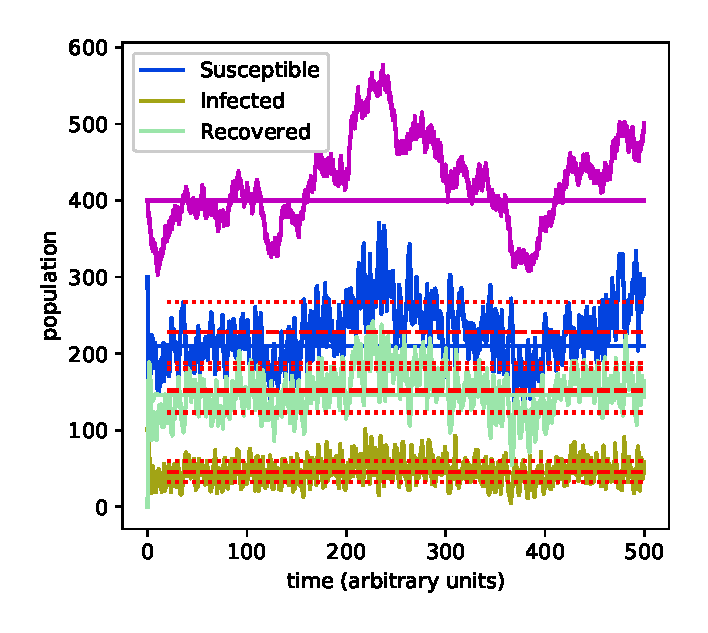
\includegraphics[width=\linewidth]{Bd01e01_1.eps}
	\small
	\begin{tabular}{c l r}
  &    Monte Carlo     &  ODE  \\\hline
S &  228.0 $\pm$  40.0 &  210.0 \\
I &   46.0 $\pm$  13.8 &   43.8 \\
R &  151.9 $\pm$  28.7 &  146.2 \\\hline
	\end{tabular}
	\caption{Evolution of population B with added parameters $\nu=\mu=0.1$. The magenta curves show the total population, and the red lines indicate the mean and standard deviation of the Monte Carlo simulation after $t=20$.} 
	\label{fig:vit}
\end{figure}




\begin{figure}
	\centering
	\begin{subfigure}{\linewidth}
		\centering
		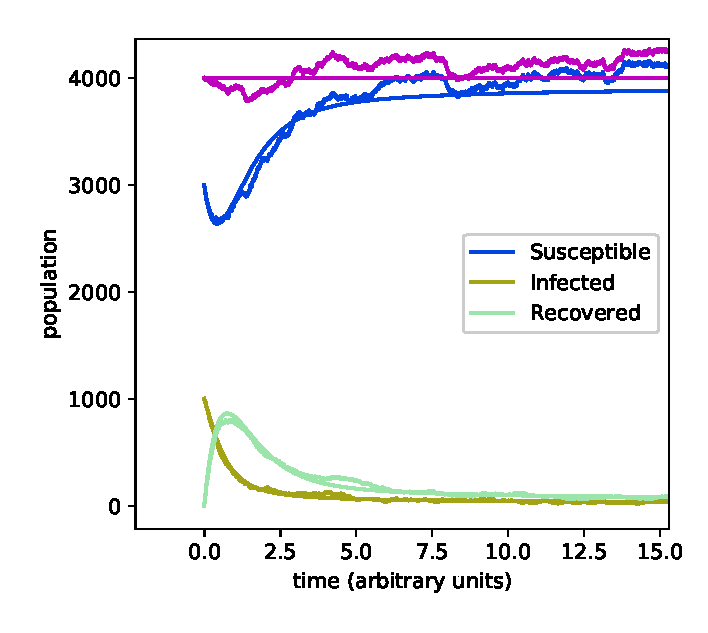
\includegraphics[width=\linewidth]{a4b3c05e09d09_x10_1.eps}
		\caption{Vital parameters $\mu=\nu=0.9$, thus $R_0=4/3.9\approx1.026$}
		\label{fig:cstay}
	\end{subfigure}
	\begin{subfigure}{\linewidth}
		\centering
		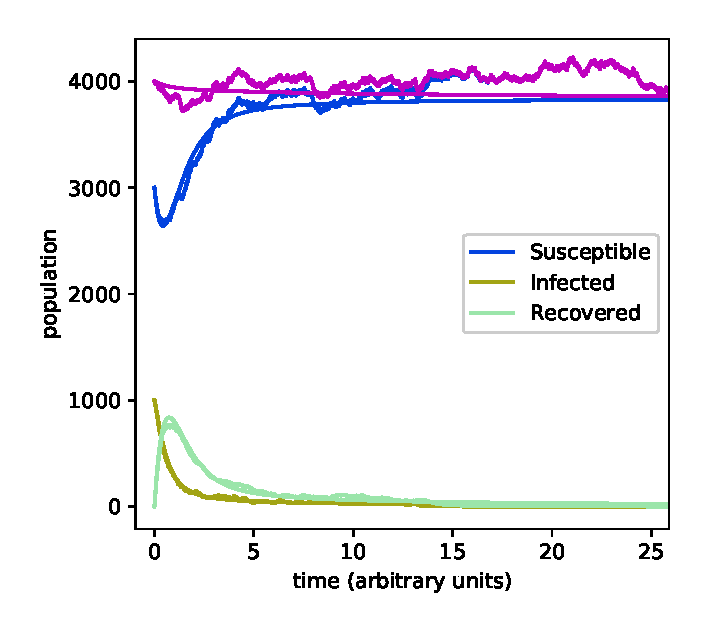
\includegraphics[width=\linewidth]{a4b3c05e09d09dI01_x10_1.eps}
		\caption{Vital parameters $\mu=\nu=0.9$ and $\mu_I=0$, thus $R_0=1$}
		\label{fig:cgon}
	\end{subfigure}
	\caption{Evolution of the system for a population equivalent to population C but ten times as large, with basic reproduction numbers slightly larger and equal to 1.}
	\label{fig:c}
\end{figure}






\begin{figure*}
	\centering
\begin{subfigure}{.5\textwidth}
	\centering
	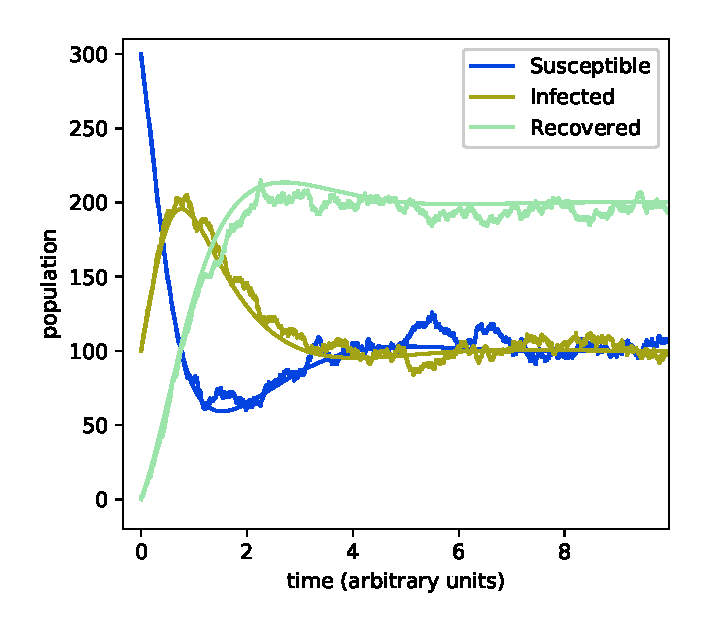
\includegraphics[width=\linewidth]{a4b1c05_1.eps}
	\small
	\begin{tabular}{c l r}
	  &    Monte Carlo   &  ODE  \\ \hline
	S &  101.1 $\pm$ 11.2 &  100.0 \\
	I &  100.6 $\pm$ 10.1 &  100.0 \\
	R &  198.3 $\pm$  9.7 &  200.0 \\\hline
	\end{tabular}
	\caption{Population A, equilibrium reached at $t_\mathrm{eq}=10$.} 
	\label{fig:aA}
\end{subfigure}%
\begin{subfigure}{.5\textwidth}
	\centering
	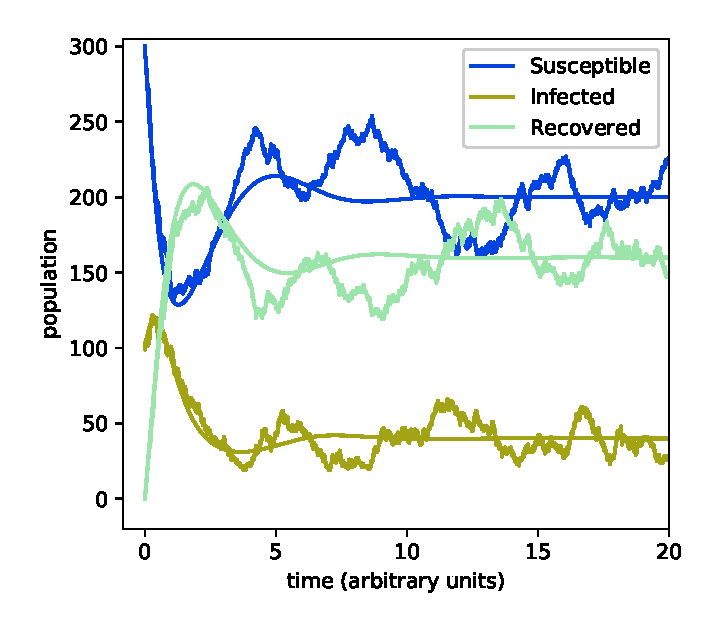
\includegraphics[width=\linewidth]{a4b2c05_1.eps}
	\small
	\begin{tabular}{c l r}
  &    Monte Carlo     &  ODE  \\\hline
S &  202.8 $\pm$  23.1 &  200.0 \\
I &   39.8 $\pm$  10.7 &   40.0 \\
R &  157.4 $\pm$  18.3 &  160.0 \\\hline
	\end{tabular}
	\caption{Population B, equilibrium reached at $t_\mathrm{eq}=20$.}
	\label{fig:aB}
\end{subfigure} 
\begin{subfigure}{.5\textwidth}
	\centering
	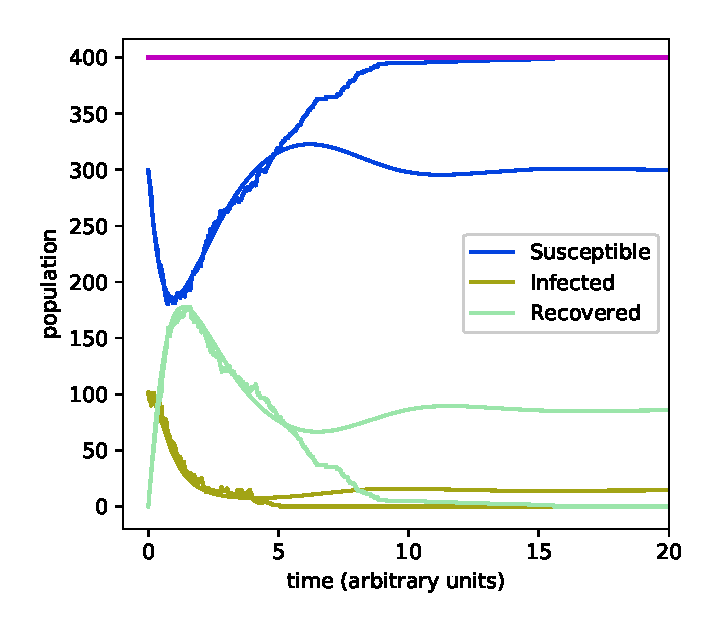
\includegraphics[width=\linewidth]{a4b3c05_1.eps}
	\small
	\begin{tabular}{c l r}
  &    Monte Carlo     &  ODE  \\\hline
S &  400.0 $\pm$   0.0 &  300.0 \\
I &    0.0 $\pm$   0.0 &   14.3 \\
R &    0.0 $\pm$   0.0 &   85.7 \\\hline
	\end{tabular}
	\caption{Population C, equilibrium reached at $t_\mathrm{eq}=20$.}
	\label{fig:aC}
\end{subfigure}%
\begin{subfigure}{.5\textwidth}
	\centering
	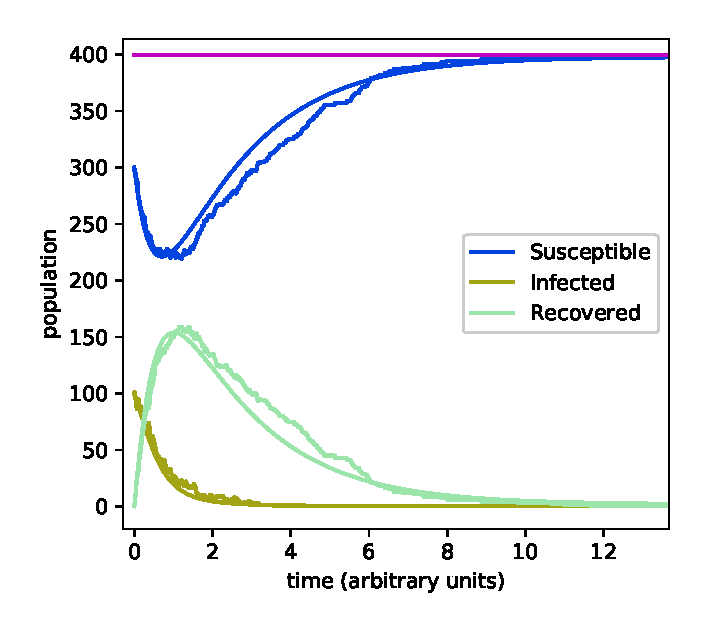
\includegraphics[width=\linewidth]{a4b4c05_1.eps}
	\small
	\begin{tabular}{c l r}
   &    Monte Carlo     &  ODE  \\\hline
S &  400.0 $\pm$   0.0 &  399.3 \\
I &    0.0 $\pm$   0.0 &    0.1 \\
R &    0.0 $\pm$   0.0 &    0.6 \\\hline
	\end{tabular}
	\caption{Population C, equilibrium reached at $t_\mathrm{eq}=20$.}
	\label{fig:aD}
\end{subfigure}
	\caption{Evolution of the model for the four the populations described in the text. The graphs show the evolution before equilibration, and the tables show the equilibrium state. The values for the Monte Carlo are means over $t\in[t_\mathrm{eq},100]$.}
	\label{fig:a} 
\end{figure*}


\begin{comment}
\begin{figure}
	\centering
	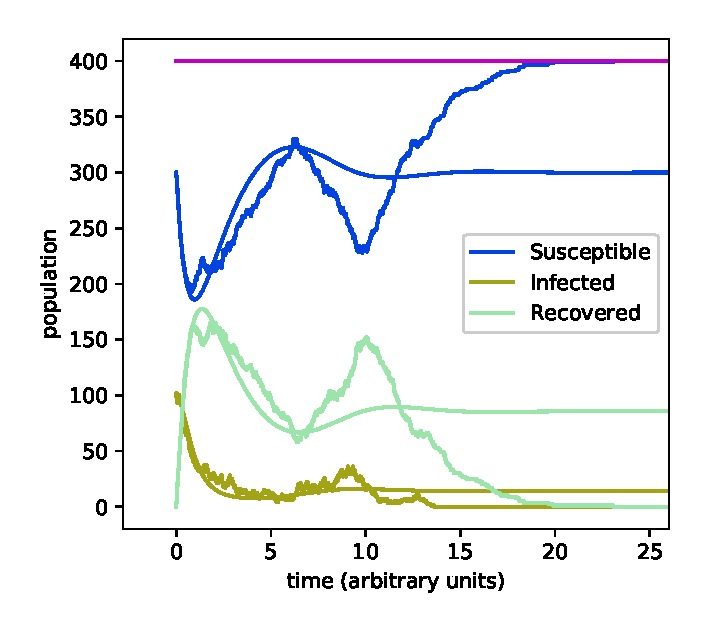
\includegraphics[width=\linewidth]{a4b3c05_n1742748670.eps}
	\caption{Evolution of the model for population C before equilibrium. The model is identical to the one shown in figure \ref{fig:aC}, but uses a different seed when generating random numbers.}
	\label{fig:C}
\end{figure}
\end{comment}







\begin{figure*}
	\centering
	\begin{subfigure}{0.5\textwidth}
		\centering
		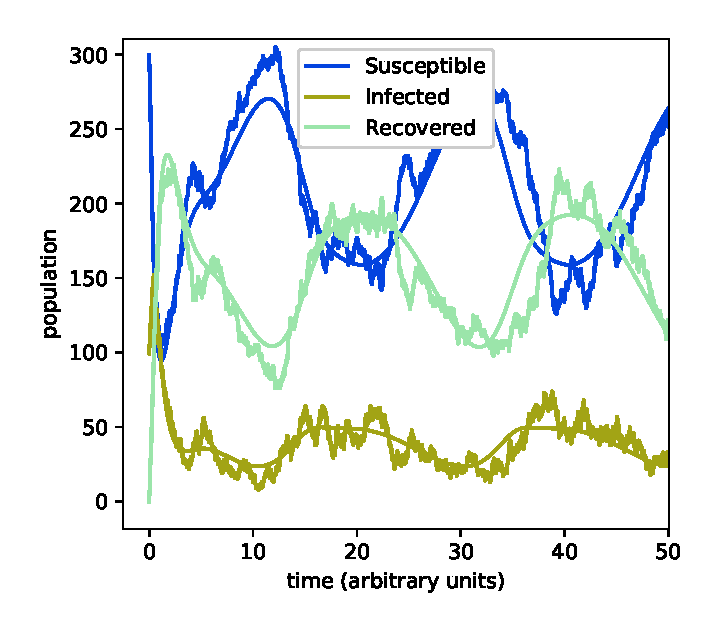
\includegraphics[width=\linewidth]{BA1w0pi_1.eps}
		\caption{$\omega = \pi/10$ : period comparable to $t_\mathrm{eq}$.}
		\label{fig:dshort}
	\end{subfigure}%
	\begin{subfigure}{0.5\textwidth}
		\centering
		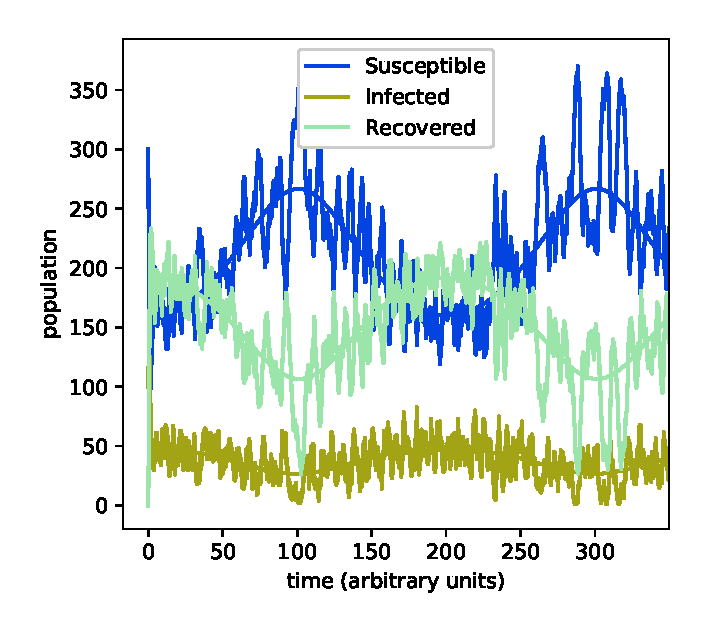
\includegraphics[width=\linewidth]{BA1w00pi_1.eps}
		\caption{$\omega = \pi/100$ : period much longer than $t_\mathrm{eq}$.}
		\label{fig:dlong}
	\end{subfigure}
	\caption{Evolution of the model for population B with time dependent transmission parameter $\beta(t)$ given by equation \ref{eq:seasvar}, using $A=1$ and different oscillation frequencies.}
	\label{fig:d}
\end{figure*}



\begin{figure*}
	\centering
\begin{subfigure}{0.5\linewidth}
	\centering
	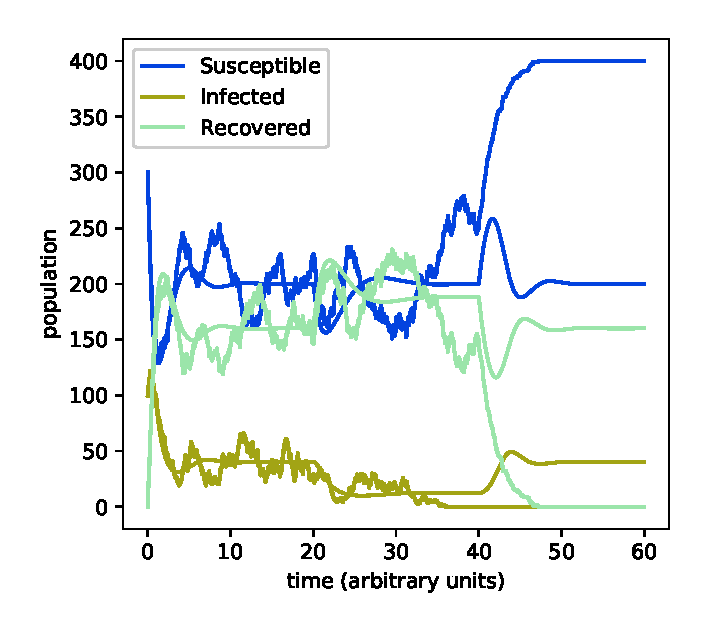
\includegraphics[width=\linewidth]{Bf70i2040_1.eps}
	\caption{Constant vaccination rate of 70 in the time interval $[20,40]$.}
	\label{fig:ecamp}
\end{subfigure}%
\begin{subfigure}{0.5\linewidth}
	\centering
	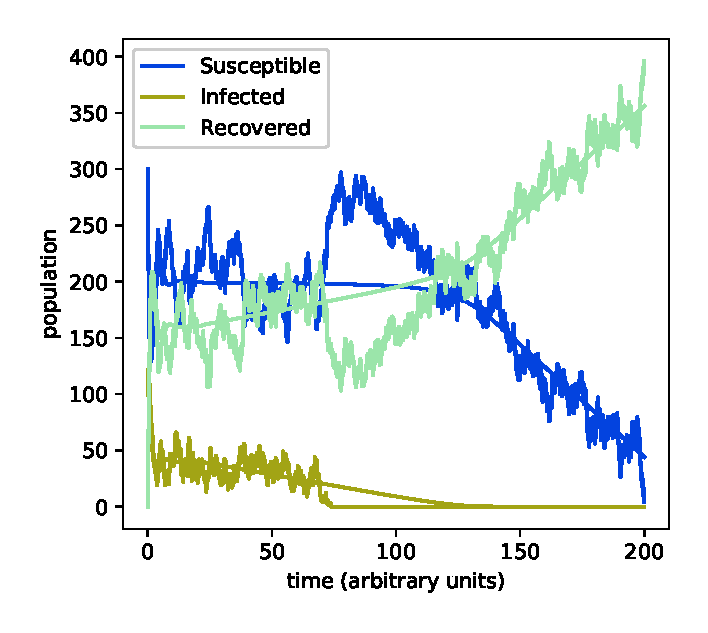
\includegraphics[width=\linewidth]{Bf1ti20inf_1.eps}
	\caption{Linearly increasing vaccination rate from $t=20$.}
	\label{fig:einc}
\end{subfigure}
	\caption{Evolution of the  model for population B when adding vaccination for two different vaccination rates $f(t)$.}
	\label{fig:e}
\end{figure*}

\begin{figure*}
	\centering
	\begin{subfigure}{0.33\linewidth}
		\centering
		\includegraphics[width=\linewidth]{SIR_early_n1975647833.eps}
	\end{subfigure}%
	\begin{subfigure}{0.33\linewidth}
		\centering
		\includegraphics[width=\linewidth]{SIR_late_n457858786.eps}
	\end{subfigure}%
	\begin{subfigure}{0.33\linewidth}
		\centering
		\includegraphics[width=\linewidth]{SIR_none_n1815345841.eps}
	\end{subfigure}%
	\caption{SIR simulations with $[S,I,R] = [399,1,9]$ at $t=0$, and parameters $\beta = 4, \gamma = 2$, for three different seeds.}
	\label{fig:seed}
\end{figure*}


	 




%
%
%
\section{Discussion}






\subsection{Impact of the studied improvements}


In accordance with expectation, we observe a change in the equilibrium values in figure \ref{fig:vit} when compared to figure \ref{fig:aB}. The proportions of $S$, $I$ and $R$ are similar for the two algorithms:
\begin{center}
\begin{tabular}{ccc}\hline
& ODE & Monte Carlo	\\\hline
S & 52.50\% & 53.53\% \\
I & 10.95\% & 10.80\% \\
R & 36.55\% & 35.66\%  \\\hline
\end{tabular}
\end{center}
The large fluctuations in the total population will be discussed in section \ref{ssec:dif}. 

For the model with vital dynamics, the basic reproduction number is found from equation \ref{eq:cI} to be 
\[
R_0 = \frac{\beta}{\gamma + \mu + \mu_I}.
\]
The impact of this threshold value is seen  in figure \ref{fig:c}. Indeed, in this scenario the lethal disease was eradicated while the non-lethal one remained in the population. 


Adding seasonal variation creates a varying equilibrium with the same period. As seen in figure \ref{fig:d}, the maximum transmission rate $\beta(t)$ corresponds to the maximum $I$ and $R$ and the minimum $S$. 
For periods much longer than the system's equilibration time, the variations are close to sinusoidal; the change is slow enough that the compartments can equilibrate almost instantaneously. This situation is shown in figure \ref{fig:dlong}.
For periods comparable to the equilibration time, as in figure \ref{fig:dshort}, the other rates also contribute to the shape of the oscillations. For instance, we see a slight delay between the maxima of $I$ and $R$, due to the recovery rate $\gamma$. 



In a simple vaccination campaign like the one modeled in figure \ref{fig:ecamp}, where we assume a constant vaccination rate, a new equilibration of the system is induced. Moving individuals from $S$ to $R$ also decreases the probability of infection $(aSI/N)\Delta t$, and increases the transition from $R$ to $S$. The net result is the equilibrium for $S$ stying the same, as observed.
If the number of infected drops low enough, fluctuations in the Monte Carlo simulation can cause it to become zero, eradicating the disease. 
The ODE algorithm will always return to the original steady state once the campaign ends, because $I$ can approach zero asymptotically.   

For the increasing vaccination rate modeled in figure \ref{fig:einc}, the entire population will eventually be vaccinated. As long as there are still infected, $S$ stays at equilibrium for the same reason as above, and the changes in $I$ and $R$ are symmetrical. Once the disease has been eradicated, the size of $S$ starts to decline linearly and symmetrically with $R$.
       

\subsection{Notable cases of deviation between the two approches}\label{ssec:dif}

As seen in figures \ref{fig:e} and \ref{fig:aC}, the two implementations differ greatly once the number of infected individuals approaches zero. 
If the $I$ is close to zero for a long  time compared to $\Delta t$, then the Monte Carlo algorithm is likely to reach zero due to random fluctuations, ending the pandemic.
 This also means the seed of the random number generator will have a large impact on the resulting behaviour. 
 This can be seen most clearly in figure \ref{fig:seed}, where the system starts off with only one infected. Here, despite the exact same parameters being used, we see three different behaviours. The differences can largely be traced back to the random infection by or recovery of that individual


The vital dynamics are extremely sensitive to the random fluctuations of the Monte Carlo algorithm. While the basic SIRS model has one steady state for a given set of parameters, there is no single steady state for the total population. If $\nu=\mu$, then the population is expected to remain constant, but has no preference for a particular value. 
In keeping with this, figure \ref{fig:vit} shows roughly constant proportions of $S$, $I$ and $R$, with large fluctuations in the total population.  



  
\subsection{Shortcomings of the model}

In many of the cases described above, the fluctuations in the Monte Carlo algorithm had a large impact on the evolution of the disease once the number of infected individuals became small. 
The ODE approach explicitly assumes populations large enough to be modeled by a continuous variable, so it cannot be used effectively in these situations. In general, statistical models are unreliable when the system is too small.
The best we can achieve with the SIRS model would be to run the Monte Carlo simulation multiple times and thus estimate a probability of the different possible outcomes. 
In practice, it might also be possible to identify such a small number of infected and make sure the disease doesn't spread.


In this project we have only implemented a few simple improvements to the standard SIRS model, and have studied different parameters without considering their realism. We will point out briefly a few of the improvements we've left out.

While we did include a seasonal variation in the transmission parameter $\beta$, it can also be reduced deliberately by for example quarantines. When fighting an epidemic, a good model for the impact of quarantines can be very useful.

In the models presented here, the transition probabilities react instantaneously to changes in the compartments.%: the probabilities are directly proportional to the size of the compartment in question. This is equivalent to assuming the 
Most visibly, the  number of recovered increases quickly from $t=0$. In reality, phenomena like disease recovery, immunity loss, birth and death do not have a constant probability. The immune reaction takes time, death usually follows prolonged sickness, and newborns don't give birth. 
This time lag can be implemented into the model by taking into account the previous states of the model when calculating the transition probabilities.      


%
%
%

\section{Conclusion}
We implemented the SIRS model for infectious diseases both as a random system with a Monte Carlo algorithm, and as coupled differential equations with the Runge-Kutta 4 algorithm. 
The codes can be expanded to include more and different transitions, allowing the model to be tailored to a given situation. We added vital dynamics, sinusoidal seasonal variation of the transmission rate, and vaccination. We then studied the results of the two algorithms for various parameters, in whose selection we prioritized illustration of different behaviours over realism. 

In most circumstances, the Monte Carlo algorithm follows the ODE solution. However, the random fluctuations sometimes cause it to eradicate the disease completely when the number of infected is close to zero. 
This illustrates the limit of a statistical model for small populations.     
 
Important improvements on the basic SIRS model which were not studied in the scope of this project include the influence of previous states of the system and the modeling of quarantines.


%\onecolumn
\begin{thebibliography}{9}

   

\bibitem{labtext}
Hjort-Jensen, Morten, (2020) \textit{Project 5, Disease Modeling}, \textsc{url: }\url{http://compphysics.github.io/ComputationalPhysics/doc/Projects/2020/Project5/DiseaseModeling/html/DiseaseModeling.html}. 

\bibitem{ODElecture}
Hjort-Jensen, Morten, (2020) \textit{Computational Physics Lectures: Ordinary differential equations}, \textsc{url: }\url{http://compphysics.github.io/ComputationalPhysics/doc/pub/ode/html/ode.html}.



\bibitem{in1900}
Langtangen, Hans Petter \& Sundnes, Joakim, (2017) \textit{App.E: Systems of differential equations}, \textsc{url: }\url{https://www.uio.no/studier/emner/matnat/ifi/IN1900/h17/ressurser/slides/ode_systems_short.pdf}

%\bibitem{primer}
%Langtangen, Hans Petter, (2016) \textit{A Primer on Scientific Programming with Python}

%\bibitem{lecture}

\bibitem{covid}
Amaro, J.E., Dudouet, J., Orce, J.N., (2020) Global analysis of the COVID-19 pandemic using simple epidemiological models, \textit{Applied Mathematical Modelling}, 90, p.995 - 1008.

\end{thebibliography}



% Husk å avslutte alle environments
% SLUTT
\end{document}